% CONCLUSIONI

\chapter{Conclusioni}\label{chap:conclusions}
\section{Valutazione del prodotto finale}
L’applicazione Teamwork sviluppata nei due mesi di stage soddisfa pienamente le aspettative dell’azienda, in quanto non pensavano di arrivare ad avere in mano un prototipo con tutte le funzionalità principali. \\
Questo ha confermato all'azienda l'effettiva utilità di un'applicazione mobile di chat da integrare nella suite Zextras. Infatti il progetto Teamwork verrà portato avanti senza applicare cambiamenti drastici dell'architettura e utilizzando il codice sviluppato nei mesi di stage.\\
La figura \ref{sec:valutazione} rappresenta tre screen dell'applicazione finale (rispettivamente login, buddylist e chat page) che possono essere confrontati con la figura \ref{subsec:wireframe} che rappresenta i wireframe progettati.
\begin{figure}[H] 
	\centering
	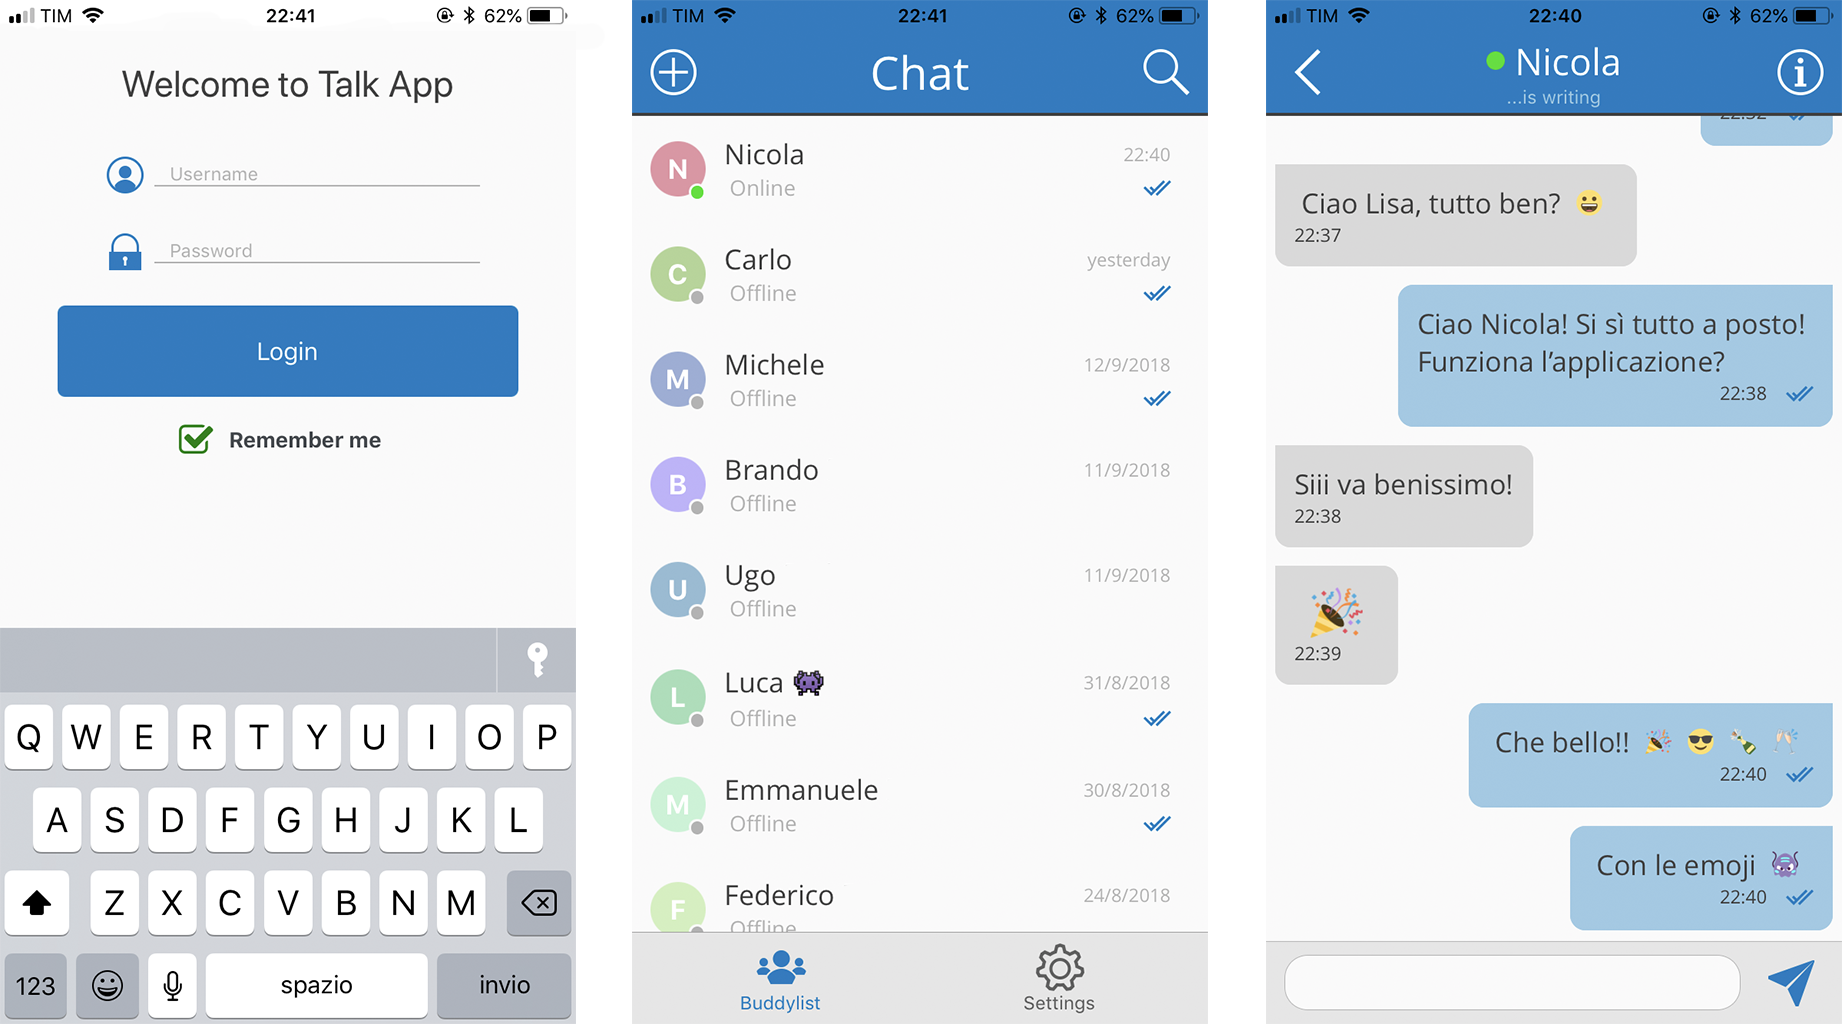
\includegraphics[scale=0.45]{screen}
	\caption{Screen pagina di login, buddylist e chat page.}
	\label{sec:valutazione}
\end{figure}
Per quanto riguarda l'interfaccia grafica sono molto soddisfatta del risultato ottenuto in quanto segue perfettamente le linee guida fornite dall'azienda. \\
Personalmente ritengo il prodotto sviluppato un ottimo prototipo della possibile applicazione chat della suite ma ancora lontana dall'essere una versione rilasciabile e testabile da utenti esterni principalmente per due motivi:
\begin{itemize}
	\item le funzionalità implementate non sono abbastanza numerose da coprire i bisogni che dovrebbe soddisfare quest'applicazione;
	\item essendo una suite di prodotti utilizzati per il lavoro bisognerebbe assicurare una certa sicurezza che in due mesi non è stata possibile raggiungere.
\end{itemize}


\section{Valutazione framework e librerie utilizzate}
L'obbiettivo di questo progetto di stage, oltre ad avere un prototipo funzionante dell'applicazione, era quello di validare delle tecnologie ancora non utilizzate dall'azienda per capire se fossero effettivamente utili allo sviluppo di futuri progetti. \\
Sebbene abbia ancora molto da imparare su queste tecnologie per poterne giudicare pregi e difetti in maniera critica, ritengo adeguato effettuare una valutazione a posteri del compimento del progetto.
\subsection{Valutazione React Native}
Per realizzare l'interfaccia utente delle ultime zimlet sviluppate dall'azienda si è utilizzato ReactJS, libreria JavaScript che ha permesso di migliorare lo sviluppo e la gestione dei dati rispetto alla precedente tecnologia utilizzata specifica per Zimbra. \\
Per la realizzazione di applicazioni mobile è disponibile una sua variante, React Native, che, sebbene molte differenze, presenta una struttura simile. \\
Proprio per mantenere una certa continuità è stato deciso di testare le funzionalità di React Native in questo progetto. \\
In base all'esperienza di sviluppo avuta ho potuto valutare React Native in base a vari punti:
\subsubsection{App multipiattaforma}
React Native permette lo sviluppo di applicazioni mobile sia Android che iOS utilizzando JavaScript. In questo modo non è necessario sviluppare due versioni dell'applicazione in due linguaggi differenti per poter pubblicare l'app nei due store (App Store e Google Store). \\
Ovviamente questa integrazione presenta anche degli aspetti negativi da valutare. Innanzitutto le piattaforme native Android ed iOS presentano molte differenze e tentare di generalizzare i comportamenti di tutti i componenti nativi risulta impossibile. Per questo motivo non sono implementati tutti i componenti che avremmo a disposizione nei due ambienti di sviluppo nativi e inoltre non è detto che un componente si comporti in modo uguale su iOS e su Android. \\
In secondo luogo React Native crea un livello di astrazione al di sopra dell’applicazione che può essere meno performante di un dialogo diretto tra applicazione nativa e sistema operativo.
\subsubsection{Virtual DOM}
Per accedere e aggiornare dinamicamente il contenuto, la struttura e lo stile dei documenti nel client web e nelle applicazioni che utilizzano WebView si utilizza il \emph{\textbf{D}ocument \textbf{O}bject \textbf{M}odel} (\acrshort{DOM}), una forma di rappresentazione dei documenti strutturati, che tenta di renderli neutrali rispetto alla lingua e alla piattaforma. React Native invece utilizza il Virtual DOM che crea una struttura dei dati in-memory, lavora per differenza e quindi aggiorna in modo efficiente la DOM visualizzata dal browser. Cosi facendo vengono renderizzato solamente i componenti che vengono modificati e non tutta la pagina.
\subsubsection{JSX e CSS}
Il framework utilizza JSX come linguagggio di markup e il CSS (in formato JSON) è limitato nelle dichiarazioni. Non è possibile quindi itilizzare estensioni come SCSS e riutilizzare stylesheet web per intero...

\subsection{Valutazione Expo}
Il tool di sviluppo per applicazioni in React Native Expo è una tecnologia completamente nuova per l'azienda, consigliata da un consulente esterno. Ho raccolto i principali benefici e svantaggi dell'utilizzo di esso.\\
Aspetti positivi:
\begin{itemize}
	\item semplifica delle operazioni comuni che non sono gestite dai componenti di React Native introducendo dei nuovi componenti Expo;
	\item si sono velocizzati di molto i tempi di testing su device fisici in quando Expo propone build automatiche nei propri server che possono essere scaricate in qualsiasi device tramite link alla build;
	\item riduce la complessità di creazione di file .apk e .ipa in quanto crea le build nei propri server e gestisce le certificazioni in autonomia.
\end{itemize}
Aspetti negativi:
\begin{itemize}
	\item l'interazione tra Expo e React Native Debugger ha riscontrato non pochi problemi che causavano spesso l'interruzione dei servizi Expo;
	\item Expo client risulta ancora molto instabile causando crash dell'applicazione;
\end{itemize}

\section{Aspetti critici e possibili estensioni del prodotto}
%Considerando inoltre che l’applicazione sviluppata non utilizza particolari ottimizzazioni si ritiene che ci sia un ulteriore margine di miglioramento.
%Per quanto riguarda l’applicazione, l’aspetto grafico è stato lasciato in secondo piano e quindi può essere migliorato, specialmente per quanto riguarda l’aspetto dei pulsanti e delle icone. Questa scelta è stata fatta dal momento che lo scopo principale dell’applicazione è quello di valutare se l’utilizzo di un framework diverso possa portare alla realizzazione di un’applicazione migliore rispetto al client per iPad attuale. L’applicazione sviluppata è quindi considerata dall’azienda come un prototipo e conseguentemente non è prevista una futura manutenzione del codice. Si è scelto di non implementare i test d’unità con Jest e di non utilizzare Flow per l’analisi statica, in quanto è stato ritenuto più interessante provare ad implementare funzionalità aggiuntive offerte dal framework come le animazioni, piuttosto che concentrarsi sulla qualità del codice. Sempre riguardo l’applicazione sviluppata, è stata implementa solamente la visualizzazione della gallery, trascurando tutte le altre funzionalità offerte dal client attuale, come ad esempio la pagina di autenticazione, la creazione di nuovi assets e la possibilità di utilizzare la parte collaborativa del sistema WARDA. Tali funzionalità non sono state analizzate e implementate per motivi di tempo.

\section{Bilancio conoscenze pregresse e acquisite}
%Durante le attività di stage sono state acquisite competenze sia nello sviluppo di applicazioni mobile, sia in altri settori ad esso correlati. Principalmente è stato studiato come è possibile sviluppare applicazioni mobile utilizzando JavaScript, sia sotto forma di applicazioni ibride che come applicazioni native, analizzando le varie strategie utilizzate per astrarre le API native dei dispositivi mobile. Inoltre, i framework analizzati durate il periodo di stage erano totalmente sconosciuti, mentre al termine dello stage sono state acquisite delle conoscenze basilari riguardo i vari framework. In particolar modo per quanto riguarda React Native è stata raggiunta una buona padronanza del framework, specialmente nello sviluppo di un’applicazione secondo i pattern tipici, anch’essi sconosciuti prima dell’inizio dello stage. Sempre legato allo sviluppo, si sono acquisite delle competenze riguardo ai tools offerti da Xcode per il debug di applicazioni native, che prima non erano mai stati utilizzati. Sono state inoltre rafforzate le competenze riguardo il linguaggio JavaScript, che era già noto prima dello stage, ma del quale non ero a conoscenza dello standard ES6 e la sintassi JSX. In secondo luogo sono state acquisite delle nozioni riguardo alcuni aspetti del mondo aziendale, in particolare si è potuto osservare come un’azienda valuta le caratteristiche di un framework per stimare i benefici e i costi derivanti dall’introduzione di tale framework nel processo di sviluppo. Inoltre è stato possibile osservare come l’esperienza utente e i feedback forniti dai clienti influiscano sulla progettazione di un’interfaccia grafica e portino ad adottare determinate strategie per massimizzare le prestazioni al fine di soddisfare le loro esigenze. Infine, utilizzando le API REST di WARDA è stato possibile osservare come viene utilizzata l’architettura REST a livello aziendale e come creare un’applicazione che utilizzi tali API.